

\section{Introduction}

Likewise, the purpose of this chapter is to go through the important theories in developing the prototype together with training and testing the machine learning model.

\section{Relevant Theories and Models}

\begin{figure}[!htbp]
	\centering
	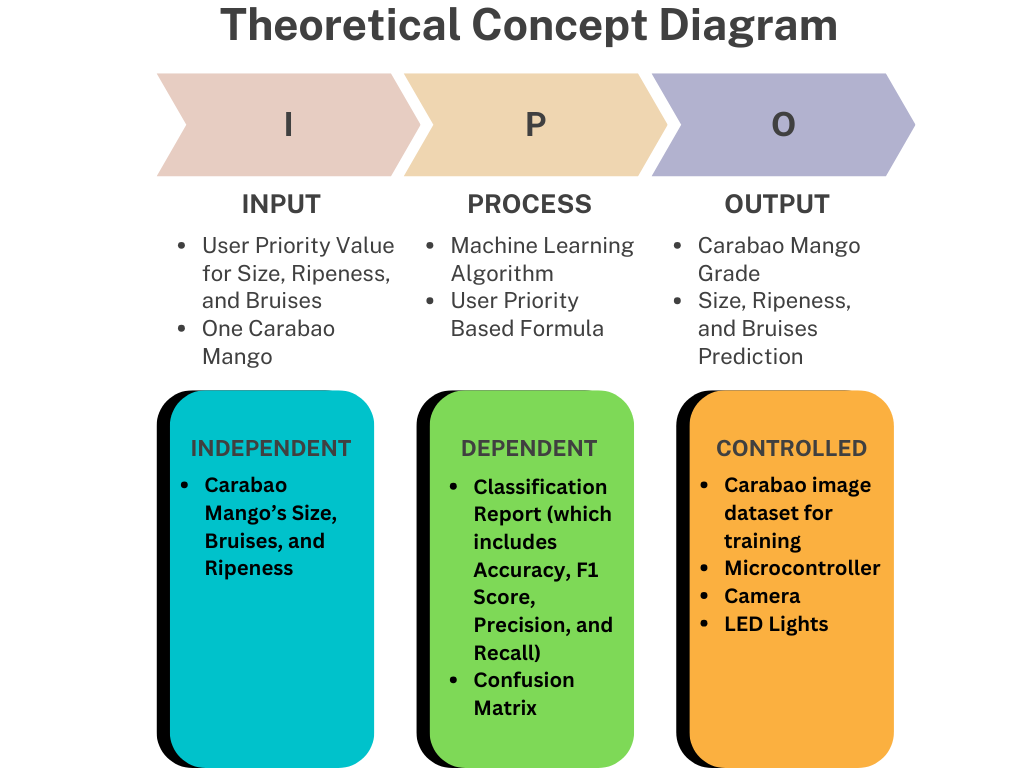
\includegraphics[width=0.5\textwidth]{theoretical_diagram3}
	\caption{Theoretical Framework Diagram.}
	\label{fig:theoreticalDiagram1}
\end{figure}


The theoretical framework seen in figure x revolves around the concepts that revolve around the research topic. 
Embedded systems include the Raspberry Pi, which is the microcontroller that will be the brain of the system, 
\gls{DC} motors, 4 channel relays, and the conveyor belt. The machine learning portion includes a neural network 
model, namely the Convolutional Neural Network, which will use computer vision as a method of seeing and classifying
 the mangoes based on their physical traits. The image processing will include methods such as size calculation and 
 background removal using OpenCV. Lastly, the Carabao mango will be the test subject of the system.

\section{Technical Background}

At its core, the system will be using machine learning concepts pertaining to \gls{CNN} and OpenCV, and may use other algorithms such as Naive Bayes and k-Nearest Neighbors to supplement the classification tasks, particularly for assessing mango ripeness, bruise detection, and size determination. The system will be built on an embedded framework, integrating a Raspberry Pi microcontroller to control the RaspberryPi camera, actuators, LED lights, and motors. A user-friendly GUI will also be utilized to ensure users can customize the prioritization of the mango sorting system.

\section{Conceptual Framework Background}

\begin{figure}[!htbp]
	\centering
	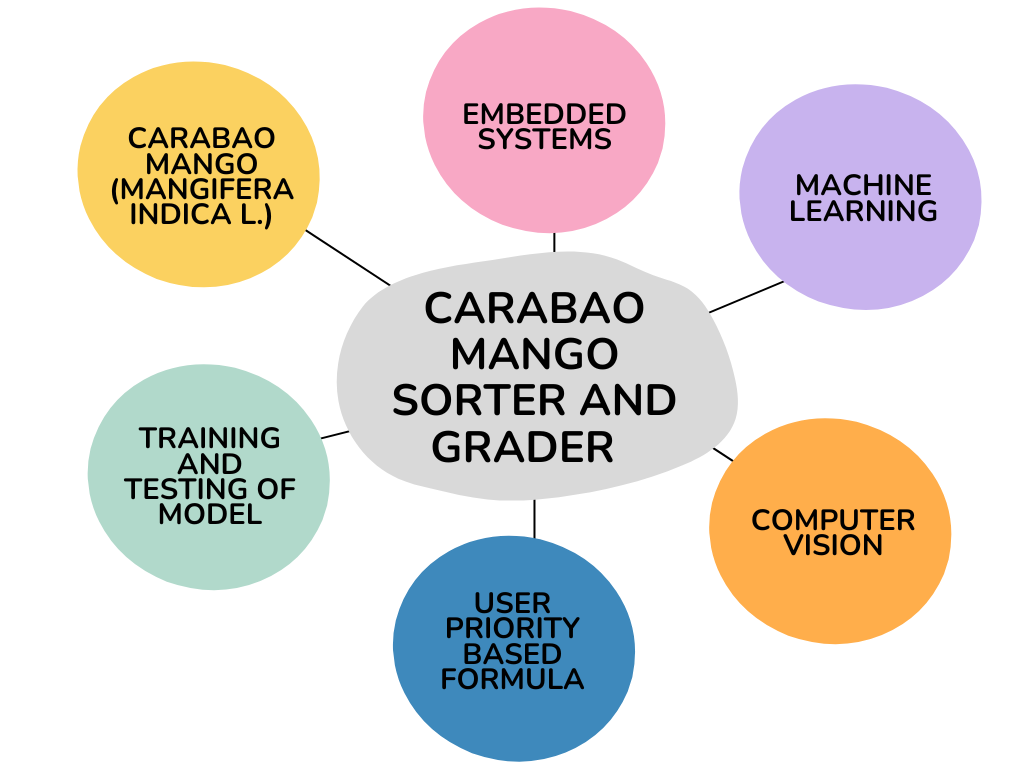
\includegraphics[width=0.5\textwidth]{concept_diagram}
	\caption{Conceptual Framework Diagram.}
	\label{fig:theoreticalDiagram2}
\end{figure}

\section{Software Concepts}

\subsection{Thresholding}
% add thresholding concept and how it is used in the system

\subsection{Object Size Calculation}
% (pixel_dimension * distance_camera_to_object) / focal_length_pixels = real_world_dimension
The size of the mango can be determined given:

\begin{equation}
	\label{eq:objectSizeCalculation}
	\text{Real World Dimension} = \frac{\text{Pixel Dimension} \times \text{Distance from Camera to Object}}{\text{Focal Length}}
\end{equation}

\begin{equation} \label{eq:objectSizeCalculation2}
	\ensuremath{D \left( p, d, f \right)= \frac{p \cdot d}{f} }
\end{equation}

where \gls{not:real_world_dimension} is the real world dimension of the object,
 \gls{not:pixel_dimension} is the pixel dimension of the object, 
 \gls{not:distance_from_cam_to_object} is the distance from the camera to the object,
  and \gls{not:focal_length} is the focal length of the camera.

\subsection{Convolutional Neural Network}
% describe CNN and show the architecture of the CNN model

\subsection{Classification Report}
% describe classification report and how it is used in the system

\subsubsection{Confusion Matrix}
\begin{table}[h]
	\centering
	\begin{tabular}{c|c|c}
	\hline
	& \textbf{Predicted Positive} & \textbf{Predicted Negative} \\
	\hline
	\textbf{Actual Positive} & TP & FN \\
	\hline
	\textbf{Actual Negative} & FP & TN \\
	\hline
	\end{tabular}
	\caption{Confusion Matrix Example}
	\label{tab:confusion_matrix}
\end{table}
A confusion matrix is a table that visualizes the performance 
of a classification model. For a binary classification problem, it has four components:
\begin{itemize}
	\item True Positives (TP): Cases correctly predicted as positive
	\item True Negatives (TN): Cases correctly predicted as negative
	\item False Positives (FP): Cases incorrectly predicted as positive. (Type I error)
	\item False Negatives (FN): Cases incorrectly predicted as negative (Type II error)
\end{itemize}

\subsubsection{Precision}
\begin{eqnarray}
	\text{Precision} = \frac{TP}{TP + FP}
	\label{eq:precision}
\end{eqnarray}

Precision measures how many of the predicted positives are actually positive. It answers the question: 
"When the model predicts the positive class, how often is it correct?" High precision means low false positives.

\subsubsection{Recall}
\begin{eqnarray}
	\text{Recall} = \frac{TP}{TP + FN}
	\label{eq:recall}
\end{eqnarray}

Recall, which is also called sensitivity, measures how many of the actual positives were correctly identified. 
It answers the question: 
"Of all the actual positive cases, how many did the model catch?" High recall means low false negatives.

\subsubsection{F1 Score}
\begin{eqnarray}
	F_1 = 2\times \frac{\text{Precision} \times \text{Recall}}{\text{Precision} + \text{Recall}}
	\label{eq:f1_score}
\end{eqnarray}

The F1 score is the harmonic mean of precision and recall. It provides a single metric that balances 
both concerns. This is particularly useful when you need to 
find a balance between precision and recall, as optimizing for one often decreases the other.

\subsubsection{Accuracy}
\begin{eqnarray}
	\text{Accuracy} = \frac{TP + TN}{TP + TN + FP + FN}
	\label{eq:accuracy}
\end{eqnarray}

Accuracy measures the proportion of correct predictions (both true positives and true negatives)
 among the total cases. While intuitive, accuracy can be misleading with imbalanced datasets.

\section{Hardware Concepts}

\subsection{Camera Module} 

\subsection{4 Channel Relay}
% add Relay H-bridge circuit diagram

\subsection{1:3 Pulley Belt}
% add picture of a pulley belt and concept behind it (what is a pulley belt)

% PUT THE FOLLOWING IN THE THEORETICAL CONSIDERATION
% H bridge type connection with the two DC motors
% 1:3 belt connection unless changed
% Stepper Motor Specifications
% https://www.makerlab-electronics.com/products/stepper-motor-nema-17-2600g-cm
% https://lastminuteengineers.com/drv8825-stepper-motor-driver-arduino-tutorial/

\section{Summary}

Overall, chapter 3 establishes key concepts and theoretical considerations that form the foundation of the Carabao mango sorter and grading system. It discusses and connects each component together, explaining how each component such as the RaspberryPi and DC motors work together to create a system that utilizes machine learning and computer vision techniques to classify mangoes based on user priority.